\documentclass[1p]{elsarticle_modified}
%\bibliographystyle{elsarticle-num}

%\usepackage[colorlinks]{hyperref}
%\usepackage{abbrmath_seonhwa} %\Abb, \Ascr, \Acal ,\Abf, \Afrak
\usepackage{amsfonts}
\usepackage{amssymb}
\usepackage{amsmath}
\usepackage{amsthm}
\usepackage{scalefnt}
\usepackage{amsbsy}
\usepackage{kotex}
\usepackage{caption}
\usepackage{subfig}
\usepackage{color}
\usepackage{graphicx}
\usepackage{xcolor} %% white, black, red, green, blue, cyan, magenta, yellow
\usepackage{float}
\usepackage{setspace}
\usepackage{hyperref}

\usepackage{tikz}
\usetikzlibrary{arrows}

\usepackage{multirow}
\usepackage{array} % fixed length table
\usepackage{hhline}

%%%%%%%%%%%%%%%%%%%%%
\makeatletter
\renewcommand*\env@matrix[1][\arraystretch]{%
	\edef\arraystretch{#1}%
	\hskip -\arraycolsep
	\let\@ifnextchar\new@ifnextchar
	\array{*\c@MaxMatrixCols c}}
\makeatother %https://tex.stackexchange.com/questions/14071/how-can-i-increase-the-line-spacing-in-a-matrix
%%%%%%%%%%%%%%%

\usepackage[normalem]{ulem}

\newcommand{\msout}[1]{\ifmmode\text{\sout{\ensuremath{#1}}}\else\sout{#1}\fi}
%SOURCE: \msout is \stkout macro in https://tex.stackexchange.com/questions/20609/strikeout-in-math-mode

\newcommand{\cancel}[1]{
	\ifmmode
	{\color{red}\msout{#1}}
	\else
	{\color{red}\sout{#1}}
	\fi
}

\newcommand{\add}[1]{
	{\color{blue}\uwave{#1}}
}

\newcommand{\replace}[2]{
	\ifmmode
	{\color{red}\msout{#1}}{\color{blue}\uwave{#2}}
	\else
	{\color{red}\sout{#1}}{\color{blue}\uwave{#2}}
	\fi
}

\newcommand{\Sol}{\mathcal{S}} %segment
\newcommand{\D}{D} %diagram
\newcommand{\A}{\mathcal{A}} %arc


%%%%%%%%%%%%%%%%%%%%%%%%%%%%%5 test

\def\sl{\operatorname{\textup{SL}}(2,\Cbb)}
\def\psl{\operatorname{\textup{PSL}}(2,\Cbb)}
\def\quan{\mkern 1mu \triangleright \mkern 1mu}

\theoremstyle{definition}
\newtheorem{thm}{Theorem}[section]
\newtheorem{prop}[thm]{Proposition}
\newtheorem{lem}[thm]{Lemma}
\newtheorem{ques}[thm]{Question}
\newtheorem{cor}[thm]{Corollary}
\newtheorem{defn}[thm]{Definition}
\newtheorem{exam}[thm]{Example}
\newtheorem{rmk}[thm]{Remark}
\newtheorem{alg}[thm]{Algorithm}

\newcommand{\I}{\sqrt{-1}}
\begin{document}

%\begin{frontmatter}
%
%\title{Boundary parabolic representations of knots up to 8 crossings}
%
%%% Group authors per affiliation:
%\author{Yunhi Cho} 
%\address{Department of Mathematics, University of Seoul, Seoul, Korea}
%\ead{yhcho@uos.ac.kr}
%
%
%\author{Seonhwa Kim} %\fnref{s_kim}}
%\address{Center for Geometry and Physics, Institute for Basic Science, Pohang, 37673, Korea}
%\ead{ryeona17@ibs.re.kr}
%
%\author{Hyuk Kim}
%\address{Department of Mathematical Sciences, Seoul National University, Seoul 08826, Korea}
%\ead{hyukkim@snu.ac.kr}
%
%\author{Seokbeom Yoon}
%\address{Department of Mathematical Sciences, Seoul National University, Seoul, 08826,  Korea}
%\ead{sbyoon15@snu.ac.kr}
%
%\begin{abstract}
%We find all boundary parabolic representation of knots up to 8 crossings.
%
%\end{abstract}
%\begin{keyword}
%    \MSC[2010] 57M25 
%\end{keyword}
%
%\end{frontmatter}

%\linenumbers
%\tableofcontents
%
\newcommand\colored[1]{\textcolor{white}{\rule[-0.35ex]{0.8em}{1.4ex}}\kern-0.8em\color{red} #1}%
%\newcommand\colored[1]{\textcolor{white}{ #1}\kern-2.17ex	\textcolor{white}{ #1}\kern-1.81ex	\textcolor{white}{ #1}\kern-2.15ex\color{red}#1	}

{\Large $\underline{10_{32}~(K10a_{55})}$}

\setlength{\tabcolsep}{10pt}
\renewcommand{\arraystretch}{1.6}
\vspace{1cm}\begin{tabular}{m{100pt}>{\centering\arraybackslash}m{274pt}}
\multirow{5}{120pt}{
	\centering
	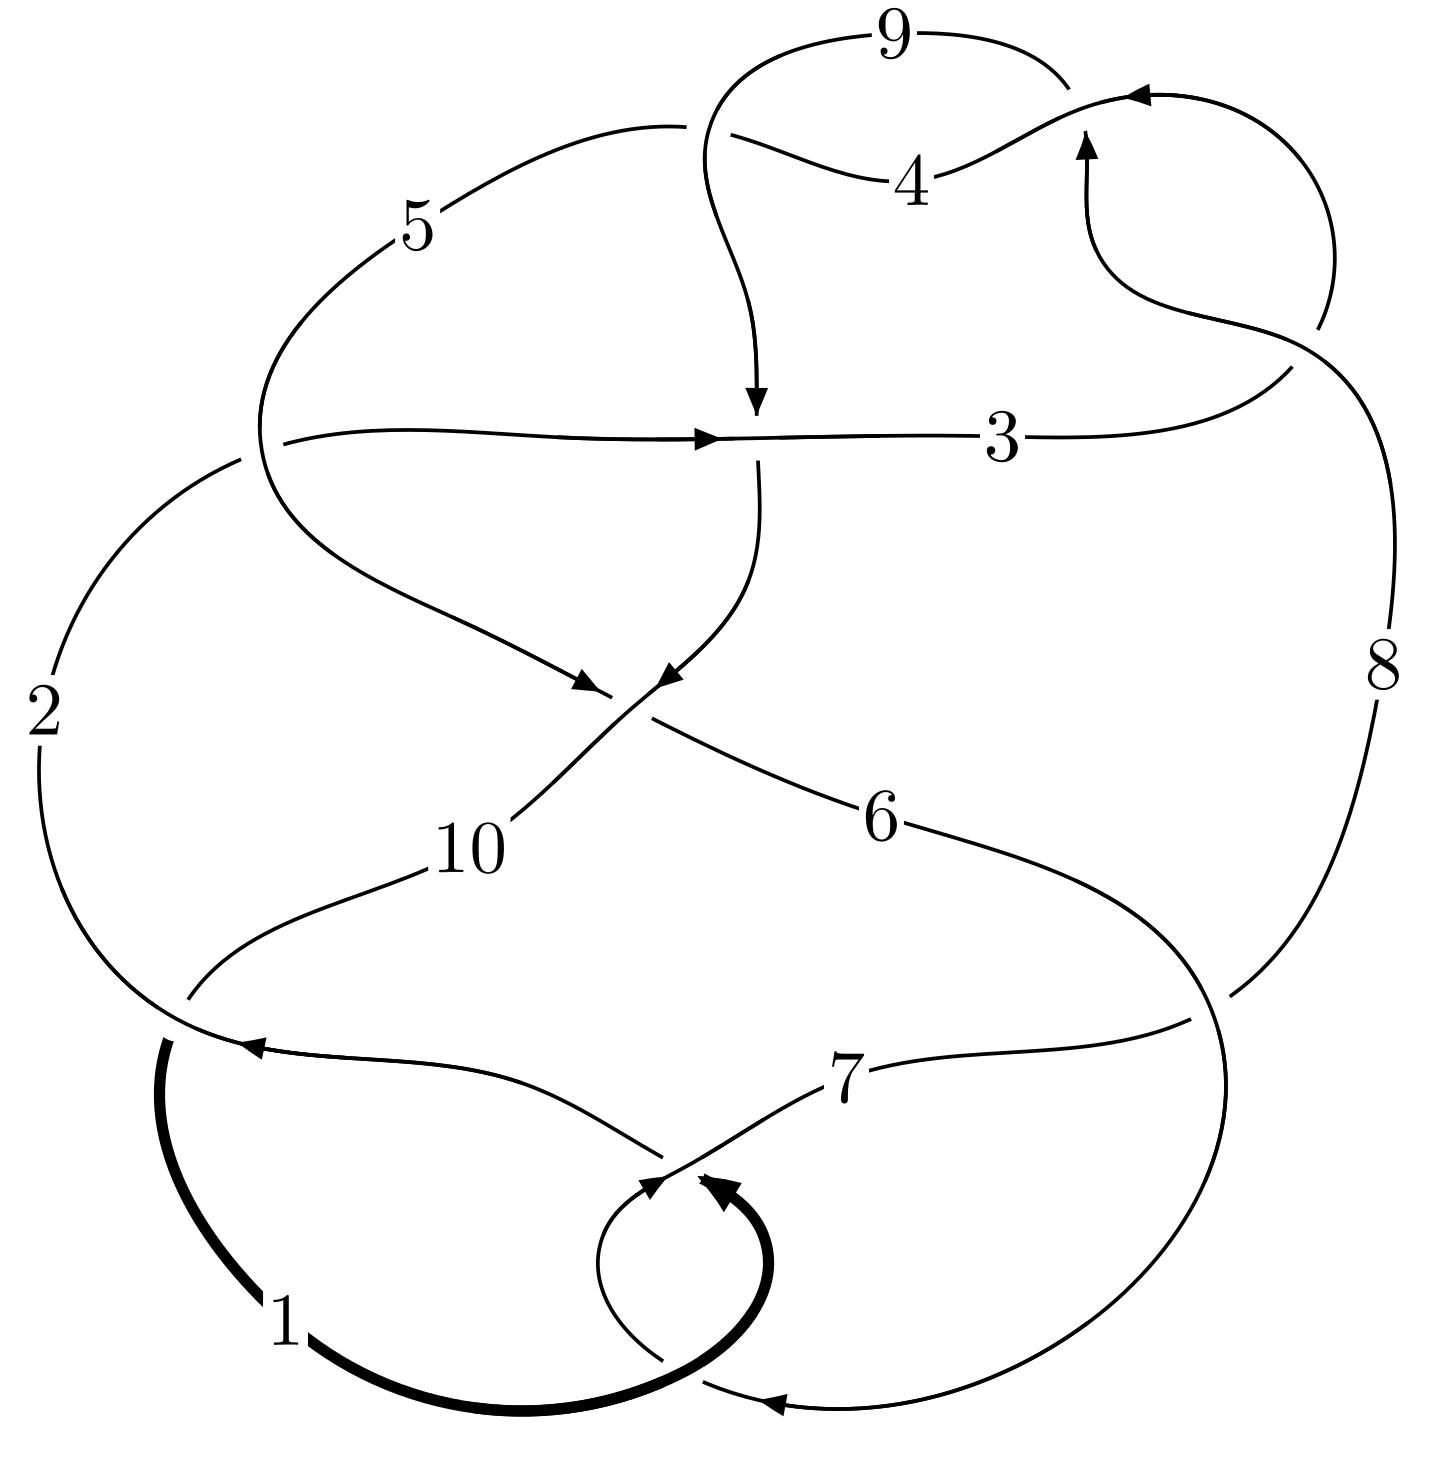
\includegraphics[width=112pt]{../../../GIT/diagram.site/Diagrams/png/116_10_32.png}\\
\ \ \ A knot diagram\footnotemark}&
\allowdisplaybreaks
\textbf{Linearized knot diagam} \\
\cline{2-2}
 &
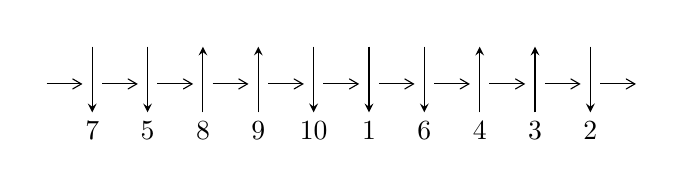
\begin{tikzpicture}[x=20pt, y=17pt]
	% nodes
	\node (C0) at (0, 0) {};
	\node (C1) at (1, 0) {};
	\node (C1U) at (1, +1) {};
	\node (C1D) at (1, -1) {7};

	\node (C2) at (2, 0) {};
	\node (C2U) at (2, +1) {};
	\node (C2D) at (2, -1) {5};

	\node (C3) at (3, 0) {};
	\node (C3U) at (3, +1) {};
	\node (C3D) at (3, -1) {8};

	\node (C4) at (4, 0) {};
	\node (C4U) at (4, +1) {};
	\node (C4D) at (4, -1) {9};

	\node (C5) at (5, 0) {};
	\node (C5U) at (5, +1) {};
	\node (C5D) at (5, -1) {10};

	\node (C6) at (6, 0) {};
	\node (C6U) at (6, +1) {};
	\node (C6D) at (6, -1) {1};

	\node (C7) at (7, 0) {};
	\node (C7U) at (7, +1) {};
	\node (C7D) at (7, -1) {6};

	\node (C8) at (8, 0) {};
	\node (C8U) at (8, +1) {};
	\node (C8D) at (8, -1) {4};

	\node (C9) at (9, 0) {};
	\node (C9U) at (9, +1) {};
	\node (C9D) at (9, -1) {3};

	\node (C10) at (10, 0) {};
	\node (C10U) at (10, +1) {};
	\node (C10D) at (10, -1) {2};
	\node (C11) at (11, 0) {};

	% arrows
	\draw[->,>={angle 60}]
	(C0) edge (C1) (C1) edge (C2) (C2) edge (C3) (C3) edge (C4) (C4) edge (C5) (C5) edge (C6) (C6) edge (C7) (C7) edge (C8) (C8) edge (C9) (C9) edge (C10) (C10) edge (C11) ;	\draw[->,>=stealth]
	(C1U) edge (C1D) (C2U) edge (C2D) (C3D) edge (C3U) (C4D) edge (C4U) (C5U) edge (C5D) (C6U) edge (C6D) (C7U) edge (C7D) (C8D) edge (C8U) (C9D) edge (C9U) (C10U) edge (C10D) ;
	\end{tikzpicture} \\
\hhline{~~} \\& 
\textbf{Solving Sequence} \\ \cline{2-2} 
 &
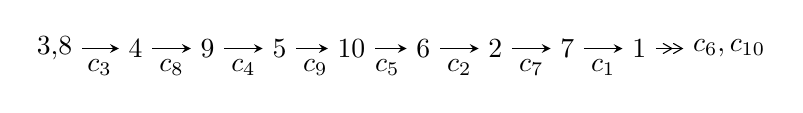
\begin{tikzpicture}[x=26pt, y=7pt]
	% node
	\node (A0) at (-1/8, 0) {3,8};
	\node (A1) at (1, 0) {4};
	\node (A2) at (2, 0) {9};
	\node (A3) at (3, 0) {5};
	\node (A4) at (4, 0) {10};
	\node (A5) at (5, 0) {6};
	\node (A6) at (6, 0) {2};
	\node (A7) at (7, 0) {7};
	\node (A8) at (8, 0) {1};
	\node (C1) at (1/2, -1) {$c_{3}$};
	\node (C2) at (3/2, -1) {$c_{8}$};
	\node (C3) at (5/2, -1) {$c_{4}$};
	\node (C4) at (7/2, -1) {$c_{9}$};
	\node (C5) at (9/2, -1) {$c_{5}$};
	\node (C6) at (11/2, -1) {$c_{2}$};
	\node (C7) at (13/2, -1) {$c_{7}$};
	\node (C8) at (15/2, -1) {$c_{1}$};
	\node (A9) at (37/4, 0) {$c_{6},c_{10}$};

	% edge
	\draw[->,>=stealth]	
	(A0) edge (A1) (A1) edge (A2) (A2) edge (A3) (A3) edge (A4) (A4) edge (A5) (A5) edge (A6) (A6) edge (A7) (A7) edge (A8) ;
	\draw[->>,>={angle 60}]	
	(A8) edge (A9);
\end{tikzpicture} \\ 

\end{tabular} \\

\footnotetext{
The image of knot diagram is generated by the software ``\textbf{Draw programme}" developed by Andrew Bartholomew(\url{http://www.layer8.co.uk/maths/draw/index.htm\#Running-draw}), where we modified some parts for our purpose(\url{https://github.com/CATsTAILs/LinksPainter}).
}\phantom \\ \newline 
\centering \textbf{Ideals for irreducible components\footnotemark of $X_{\text{par}}$} 
 
\begin{align*}
I^u_{1}&=\langle 
u^{33}-2 u^{32}+\cdots+u^2+1\rangle \\
I^u_{2}&=\langle 
u+1\rangle \\
\\
\end{align*}
\raggedright * 2 irreducible components of $\dim_{\mathbb{C}}=0$, with total 34 representations.\\
\footnotetext{All coefficients of polynomials are rational numbers. But the coefficients are sometimes approximated in decimal forms when there is not enough margin.}
\newpage
\renewcommand{\arraystretch}{1}
\centering \section*{I. $I^u_{1}= \langle u^{33}-2 u^{32}+\cdots+u^2+1 \rangle$}
\flushleft \textbf{(i) Arc colorings}\\
\begin{tabular}{m{7pt} m{180pt} m{7pt} m{180pt} }
\flushright $a_{3}=$&$\begin{pmatrix}1\\0\end{pmatrix}$ \\
\flushright $a_{8}=$&$\begin{pmatrix}0\\u\end{pmatrix}$ \\
\flushright $a_{4}=$&$\begin{pmatrix}1\\- u^2\end{pmatrix}$ \\
\flushright $a_{9}=$&$\begin{pmatrix}u\\- u^3+u\end{pmatrix}$ \\
\flushright $a_{5}=$&$\begin{pmatrix}- u^2+1\\u^4-2 u^2\end{pmatrix}$ \\
\flushright $a_{10}=$&$\begin{pmatrix}- u^3+2 u\\- u^3+u\end{pmatrix}$ \\
\flushright $a_{6}=$&$\begin{pmatrix}- u^{10}+5 u^8-8 u^6+3 u^4+u^2+1\\- u^{10}+4 u^8-5 u^6+2 u^4- u^2\end{pmatrix}$ \\
\flushright $a_{2}=$&$\begin{pmatrix}u^6-3 u^4+2 u^2+1\\- u^8+4 u^6-4 u^4\end{pmatrix}$ \\
\flushright $a_{7}=$&$\begin{pmatrix}u^{21}-10 u^{19}+\cdots+2 u^3+u\\u^{21}-9 u^{19}+33 u^{17}-62 u^{15}+62 u^{13}-33 u^{11}+13 u^9-6 u^7+u^5- u^3+u\end{pmatrix}$ \\
\flushright $a_{1}=$&$\begin{pmatrix}u^{17}-8 u^{15}+25 u^{13}-36 u^{11}+19 u^9+4 u^7-2 u^5-4 u^3+u\\- u^{19}+9 u^{17}-32 u^{15}+55 u^{13}-43 u^{11}+9 u^9+4 u^5- u^3+u\end{pmatrix}$\\&\end{tabular}
\flushleft \textbf{(ii) Obstruction class $= -1$}\\~\\
\flushleft \textbf{(iii) Cusp Shapes $= 4 u^{31}-56 u^{29}-4 u^{28}+344 u^{27}+52 u^{26}-1204 u^{25}-292 u^{24}+2600 u^{23}+912 u^{22}-3476 u^{21}-1692 u^{20}+2672 u^{19}+1824 u^{18}-912 u^{17}-1016 u^{16}+40 u^{15}+276 u^{14}-156 u^{13}-260 u^{12}+144 u^{11}+276 u^{10}+24 u^9-48 u^8-16 u^7-12 u^6+16 u^5-8 u^4-20 u^3-8 u^2-4 u-6$}\\~\\
\newpage\renewcommand{\arraystretch}{1}
\flushleft \textbf{(iv) u-Polynomials at the component}\newline \\
\begin{tabular}{m{50pt}|m{274pt}}
Crossings & \hspace{64pt}u-Polynomials at each crossing \\
\hline $$\begin{aligned}c_{1},c_{6}\end{aligned}$$&$\begin{aligned}
&u^{33}-2 u^{32}+\cdots-2 u+1
\end{aligned}$\\
\hline $$\begin{aligned}c_{2}\end{aligned}$$&$\begin{aligned}
&u^{33}-6 u^{32}+\cdots+128 u-23
\end{aligned}$\\
\hline $$\begin{aligned}c_{3},c_{4},c_{8}\end{aligned}$$&$\begin{aligned}
&u^{33}-2 u^{32}+\cdots+u^2+1
\end{aligned}$\\
\hline $$\begin{aligned}c_{5}\end{aligned}$$&$\begin{aligned}
&u^{33}+u^{31}+\cdots-8 u+1
\end{aligned}$\\
\hline $$\begin{aligned}c_{7},c_{10}\end{aligned}$$&$\begin{aligned}
&u^{33}+10 u^{32}+\cdots-2 u+1
\end{aligned}$\\
\hline $$\begin{aligned}c_{9}\end{aligned}$$&$\begin{aligned}
&u^{33}+3 u^{32}+\cdots+32 u+7
\end{aligned}$\\
\hline
\end{tabular}\\~\\
\newpage\renewcommand{\arraystretch}{1}
\flushleft \textbf{(v) Riley Polynomials at the component}\newline \\
\begin{tabular}{m{50pt}|m{274pt}}
Crossings & \hspace{64pt}Riley Polynomials at each crossing \\
\hline $$\begin{aligned}c_{1},c_{6}\end{aligned}$$&$\begin{aligned}
&y^{33}-10 y^{32}+\cdots-2 y-1
\end{aligned}$\\
\hline $$\begin{aligned}c_{2}\end{aligned}$$&$\begin{aligned}
&y^{33}+14 y^{32}+\cdots-2062 y-529
\end{aligned}$\\
\hline $$\begin{aligned}c_{3},c_{4},c_{8}\end{aligned}$$&$\begin{aligned}
&y^{33}-30 y^{32}+\cdots-2 y-1
\end{aligned}$\\
\hline $$\begin{aligned}c_{5}\end{aligned}$$&$\begin{aligned}
&y^{33}+2 y^{32}+\cdots-2 y-1
\end{aligned}$\\
\hline $$\begin{aligned}c_{7},c_{10}\end{aligned}$$&$\begin{aligned}
&y^{33}+26 y^{32}+\cdots+6 y-1
\end{aligned}$\\
\hline $$\begin{aligned}c_{9}\end{aligned}$$&$\begin{aligned}
&y^{33}-3 y^{32}+\cdots+394 y-49
\end{aligned}$\\
\hline
\end{tabular}\\~\\
\newpage\flushleft \textbf{(vi) Complex Volumes and Cusp Shapes}
$$\begin{array}{c|c|c}  
\text{Solutions to }I^u_{1}& \I (\text{vol} + \sqrt{-1}CS) & \text{Cusp shape}\\
 \hline 
\begin{aligned}
u &= -1.145930 + 0.199234 I\end{aligned}
 & \phantom{-}2.02163 - 5.40417 I & -1.16809 + 6.21521 I \\ \hline\begin{aligned}
u &= -1.145930 - 0.199234 I\end{aligned}
 & \phantom{-}2.02163 + 5.40417 I & -1.16809 - 6.21521 I \\ \hline\begin{aligned}
u &= \phantom{-}1.226990 + 0.119877 I\end{aligned}
 & \phantom{-}2.93624 + 0.57729 I & \phantom{-}                -6
1.088687 + 0. 10   I\phantom{ +0.000000I} \\ \hline\begin{aligned}
u &= \phantom{-}1.226990 - 0.119877 I\end{aligned}
 & \phantom{-}2.93624 - 0.57729 I & \phantom{-}                -6
1.088687 + 0. 10   I\phantom{ +0.000000I} \\ \hline\begin{aligned}
u &= -0.313132 + 0.699748 I\end{aligned}
 & \phantom{-}1.61043 - 8.54919 I & -1.81653 + 8.15424 I \\ \hline\begin{aligned}
u &= -0.313132 - 0.699748 I\end{aligned}
 & \phantom{-}1.61043 + 8.54919 I & -1.81653 - 8.15424 I \\ \hline\begin{aligned}
u &= \phantom{-}0.325114 + 0.672913 I\end{aligned}
 & \phantom{-}2.49948 + 2.85888 I & \phantom{-}0.03469 - 3.31371 I \\ \hline\begin{aligned}
u &= \phantom{-}0.325114 - 0.672913 I\end{aligned}
 & \phantom{-}2.49948 - 2.85888 I & \phantom{-}0.03469 + 3.31371 I \\ \hline\begin{aligned}
u &= -0.592603 + 0.413344 I\end{aligned}
 & \phantom{-}2.74796 + 4.66940 I & \phantom{-}0.86326 - 2.61989 I \\ \hline\begin{aligned}
u &= -0.592603 - 0.413344 I\end{aligned}
 & \phantom{-}2.74796 - 4.66940 I & \phantom{-}0.86326 + 2.61989 I \\ \hline\begin{aligned}
u &= -0.225806 + 0.667717 I\end{aligned}
 & -3.60419 - 3.13953 I & -8.34254 + 5.36114 I \\ \hline\begin{aligned}
u &= -0.225806 - 0.667717 I\end{aligned}
 & -3.60419 + 3.13953 I & -8.34254 - 5.36114 I \\ \hline\begin{aligned}
u &= \phantom{-}0.529781 + 0.441659 I\end{aligned}
 & \phantom{-}3.40197 + 0.91195 I & \phantom{-}2.34870 - 3.13722 I \\ \hline\begin{aligned}
u &= \phantom{-}0.529781 - 0.441659 I\end{aligned}
 & \phantom{-}3.40197 - 0.91195 I & \phantom{-}2.34870 + 3.13722 I \\ \hline\begin{aligned}
u &= \phantom{-}1.323560 + 0.186117 I\end{aligned}
 & \phantom{-}3.02759 + 0.73587 I & -0.673126 + 0.769843 I \\ \hline\begin{aligned}
u &= \phantom{-}1.323560 - 0.186117 I\end{aligned}
 & \phantom{-}3.02759 - 0.73587 I & -0.673126 - 0.769843 I \\ \hline\begin{aligned}
u &= -0.065742 + 0.645142 I\end{aligned}
 & -1.19428 + 2.21654 I & -6.16344 - 2.48417 I \\ \hline\begin{aligned}
u &= -0.065742 - 0.645142 I\end{aligned}
 & -1.19428 - 2.21654 I & -6.16344 + 2.48417 I \\ \hline\begin{aligned}
u &= -0.596679\phantom{ +0.000000I}\end{aligned}
 & -1.73897\phantom{ +0.000000I} & -4.71290\phantom{ +0.000000I} \\ \hline\begin{aligned}
u &= \phantom{-}1.387740 + 0.260179 I\end{aligned}
 & \phantom{-}1.53217 + 6.51294 I & -2.89383 - 5.98872 I \\ \hline\begin{aligned}
u &= \phantom{-}1.387740 - 0.260179 I\end{aligned}
 & \phantom{-}1.53217 - 6.51294 I & -2.89383 + 5.98872 I \\ \hline\begin{aligned}
u &= -1.396540 + 0.216616 I\end{aligned}
 & \phantom{-}5.26725 - 4.07711 I & \phantom{-}4.72201 + 3.88410 I \\ \hline\begin{aligned}
u &= -1.396540 - 0.216616 I\end{aligned}
 & \phantom{-}5.26725 + 4.07711 I & \phantom{-}4.72201 - 3.88410 I \\ \hline\begin{aligned}
u &= \phantom{-}0.245019 + 0.527971 I\end{aligned}
 & \phantom{-}0.007405 + 1.282000 I & -0.00329 - 5.16805 I \\ \hline\begin{aligned}
u &= \phantom{-}0.245019 - 0.527971 I\end{aligned}
 & \phantom{-}0.007405 - 1.282000 I & -0.00329 + 5.16805 I \\ \hline\begin{aligned}
u &= -1.42908 + 0.26025 I\end{aligned}
 & \phantom{-}8.11565 - 6.26770 I & \phantom{-}4.18982 + 3.24511 I \\ \hline\begin{aligned}
u &= -1.42908 - 0.26025 I\end{aligned}
 & \phantom{-}8.11565 + 6.26770 I & \phantom{-}4.18982 - 3.24511 I \\ \hline\begin{aligned}
u &= \phantom{-}1.44655 + 0.13460 I\end{aligned}
 & \phantom{-}9.14238 - 2.78863 I & \phantom{-}4.90822 + 2.57820 I \\ \hline\begin{aligned}
u &= \phantom{-}1.44655 - 0.13460 I\end{aligned}
 & \phantom{-}9.14238 + 2.78863 I & \phantom{-}4.90822 - 2.57820 I \\ \hline\begin{aligned}
u &= \phantom{-}1.42746 + 0.27209 I\end{aligned}
 & \phantom{-}7.18048 + 12.09090 I & \phantom{-}2.43573 - 8.11579 I\\
 \hline 
 \end{array}$$\newpage$$\begin{array}{c|c|c}  
\text{Solutions to }I^u_{1}& \I (\text{vol} + \sqrt{-1}CS) & \text{Cusp shape}\\
 \hline 
\begin{aligned}
u &= \phantom{-}1.42746 - 0.27209 I\end{aligned}
 & \phantom{-}7.18048 - 12.09090 I & \phantom{-}2.43573 + 8.11579 I \\ \hline\begin{aligned}
u &= -1.44503 + 0.15402 I\end{aligned}
 & \phantom{-}9.63768 - 3.04389 I & \phantom{-}5.82618 + 2.90426 I \\ \hline\begin{aligned}
u &= -1.44503 - 0.15402 I\end{aligned}
 & \phantom{-}9.63768 + 3.04389 I & \phantom{-}5.82618 - 2.90426 I\\
 \hline 
 \end{array}$$\newpage\newpage\renewcommand{\arraystretch}{1}
\centering \section*{II. $I^u_{2}= \langle u+1 \rangle$}
\flushleft \textbf{(i) Arc colorings}\\
\begin{tabular}{m{7pt} m{180pt} m{7pt} m{180pt} }
\flushright $a_{3}=$&$\begin{pmatrix}1\\0\end{pmatrix}$ \\
\flushright $a_{8}=$&$\begin{pmatrix}0\\-1\end{pmatrix}$ \\
\flushright $a_{4}=$&$\begin{pmatrix}1\\-1\end{pmatrix}$ \\
\flushright $a_{9}=$&$\begin{pmatrix}-1\\0\end{pmatrix}$ \\
\flushright $a_{5}=$&$\begin{pmatrix}0\\-1\end{pmatrix}$ \\
\flushright $a_{10}=$&$\begin{pmatrix}-1\\0\end{pmatrix}$ \\
\flushright $a_{6}=$&$\begin{pmatrix}1\\-1\end{pmatrix}$ \\
\flushright $a_{2}=$&$\begin{pmatrix}1\\-1\end{pmatrix}$ \\
\flushright $a_{7}=$&$\begin{pmatrix}-1\\0\end{pmatrix}$ \\
\flushright $a_{1}=$&$\begin{pmatrix}0\\-1\end{pmatrix}$\\&\end{tabular}
\flushleft \textbf{(ii) Obstruction class $= -1$}\\~\\
\flushleft \textbf{(iii) Cusp Shapes $= -6$}\\~\\
\newpage\renewcommand{\arraystretch}{1}
\flushleft \textbf{(iv) u-Polynomials at the component}\newline \\
\begin{tabular}{m{50pt}|m{274pt}}
Crossings & \hspace{64pt}u-Polynomials at each crossing \\
\hline $$\begin{aligned}c_{1},c_{3},c_{4}\\c_{5},c_{6},c_{7}\\c_{8},c_{10}\end{aligned}$$&$\begin{aligned}
&u+1
\end{aligned}$\\
\hline $$\begin{aligned}c_{2}\end{aligned}$$&$\begin{aligned}
&u-1
\end{aligned}$\\
\hline $$\begin{aligned}c_{9}\end{aligned}$$&$\begin{aligned}
&u
\end{aligned}$\\
\hline
\end{tabular}\\~\\
\newpage\renewcommand{\arraystretch}{1}
\flushleft \textbf{(v) Riley Polynomials at the component}\newline \\
\begin{tabular}{m{50pt}|m{274pt}}
Crossings & \hspace{64pt}Riley Polynomials at each crossing \\
\hline $$\begin{aligned}c_{1},c_{2},c_{3}\\c_{4},c_{5},c_{6}\\c_{7},c_{8},c_{10}\end{aligned}$$&$\begin{aligned}
&y-1
\end{aligned}$\\
\hline $$\begin{aligned}c_{9}\end{aligned}$$&$\begin{aligned}
&y
\end{aligned}$\\
\hline
\end{tabular}\\~\\
\newpage\flushleft \textbf{(vi) Complex Volumes and Cusp Shapes}
$$\begin{array}{c|c|c}  
\text{Solutions to }I^u_{2}& \I (\text{vol} + \sqrt{-1}CS) & \text{Cusp shape}\\
 \hline 
\begin{aligned}
u &= -1.00000\phantom{ +0.000000I}\end{aligned}
 & -1.64493\phantom{ +0.000000I} & -6.00000\phantom{ +0.000000I}\\
 \hline 
 \end{array}$$\newpage
\newpage\renewcommand{\arraystretch}{1}
\centering \section*{ III. u-Polynomials}
\begin{tabular}{m{50pt}|m{274pt}}
Crossings & \hspace{64pt}u-Polynomials at each crossing \\
\hline $$\begin{aligned}c_{1},c_{6}\end{aligned}$$&$\begin{aligned}
&(u+1)(u^{33}-2 u^{32}+\cdots-2 u+1)
\end{aligned}$\\
\hline $$\begin{aligned}c_{2}\end{aligned}$$&$\begin{aligned}
&(u-1)(u^{33}-6 u^{32}+\cdots+128 u-23)
\end{aligned}$\\
\hline $$\begin{aligned}c_{3},c_{4},c_{8}\end{aligned}$$&$\begin{aligned}
&(u+1)(u^{33}-2 u^{32}+\cdots+u^2+1)
\end{aligned}$\\
\hline $$\begin{aligned}c_{5}\end{aligned}$$&$\begin{aligned}
&(u+1)(u^{33}+u^{31}+\cdots-8 u+1)
\end{aligned}$\\
\hline $$\begin{aligned}c_{7},c_{10}\end{aligned}$$&$\begin{aligned}
&(u+1)(u^{33}+10 u^{32}+\cdots-2 u+1)
\end{aligned}$\\
\hline $$\begin{aligned}c_{9}\end{aligned}$$&$\begin{aligned}
&u(u^{33}+3 u^{32}+\cdots+32 u+7)
\end{aligned}$\\
\hline
\end{tabular}\newpage\renewcommand{\arraystretch}{1}
\centering \section*{ IV. Riley Polynomials}
\begin{tabular}{m{50pt}|m{274pt}}
Crossings & \hspace{64pt}Riley Polynomials at each crossing \\
\hline $$\begin{aligned}c_{1},c_{6}\end{aligned}$$&$\begin{aligned}
&(y-1)(y^{33}-10 y^{32}+\cdots-2 y-1)
\end{aligned}$\\
\hline $$\begin{aligned}c_{2}\end{aligned}$$&$\begin{aligned}
&(y-1)(y^{33}+14 y^{32}+\cdots-2062 y-529)
\end{aligned}$\\
\hline $$\begin{aligned}c_{3},c_{4},c_{8}\end{aligned}$$&$\begin{aligned}
&(y-1)(y^{33}-30 y^{32}+\cdots-2 y-1)
\end{aligned}$\\
\hline $$\begin{aligned}c_{5}\end{aligned}$$&$\begin{aligned}
&(y-1)(y^{33}+2 y^{32}+\cdots-2 y-1)
\end{aligned}$\\
\hline $$\begin{aligned}c_{7},c_{10}\end{aligned}$$&$\begin{aligned}
&(y-1)(y^{33}+26 y^{32}+\cdots+6 y-1)
\end{aligned}$\\
\hline $$\begin{aligned}c_{9}\end{aligned}$$&$\begin{aligned}
&y(y^{33}-3 y^{32}+\cdots+394 y-49)
\end{aligned}$\\
\hline
\end{tabular}
\vskip 2pc
\end{document}